\usecaseristoratore{Visualizzazione notifica nuovo ordine}
\label{usecase:Visualizzazione notifica nuovo ordine}

\begin{figure}[h]
	\centering
	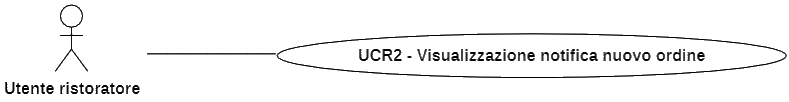
\includegraphics[width=0.9\textwidth]{./uml/UCR2.png} 
	\caption{Visualizzazione notifica nuovo ordine}
	\label{fig:UCR2}
  \end{figure}

\begin{itemize}
	\item \textbf{Attore principale:} Utente ristoratore.

	\item \textbf{Precondizione:} L'Utente base ha confermato l'ordinazione collaborativa dei pasti(vedi \autoref{usecase:Creazione dell'ordinazione collaborativa dei pasti}).

	\item \textbf{Postcondizione:} L'Utente ristoratore visualizza la notifica relativa ad una nuova ordinazione.

	\item \textbf{Scenario principale:}
	      \begin{enumerate}
		      \item Il Sistema vede che al suo interno è stata fatta una nuova ordinazione;
		      \item Il Sistema invia all'Utente ristoratore la notifica di una nuova ordinazione;
		      \item L'Utente ristoratore visualizza la notifica relativa ad una nuova ordinazione.
	      \end{enumerate}
\end{itemize}
